This chapter focuses on the modelling of the atomic elements of the robot. We begin by explaining how to create the model of an object inside V-Rep. We then show how to use to model simple elements such as frames or electronics who are not active during the simulation i.e they do not perform any function. Those can be represented strictly mechanically. We finally show how to model active pieces such as the cameras of the servos.

\section{Problem statement}
Our robot will be made from a number of elements that all need to be represented in the simulation :\begin{itemize}
\item \textbf{Miscellaneous mechanics and electronics:} A type of element that must be included in the model are the frames, \Cref{fig:fr07-h101} shows the FR07-H101 frame. On the actual robot, they will link the servos together. Other mechanical elements are the hands, the feet and the plate that will act as the trunk of the robot. 

In addition to all the aforementioned elements we plan to equip the legs of the robot with springs. Their purpose will be to 

The robot will also have some an array of electronic elements. A motherboard (\Cref{fig:odroid}) to give orders to the servos, batteries to stock the energy necessary to power them and the electronics to convey that energy through the robot.

\item \textbf{Cameras:} The robot will be equipped with two cameras of the type shown in \Cref{fig:li_cam}. They will be used by the robot to locate itself in the play arena. As we may test some machine vision algorithms during our (future) simulations we need to have the ability of retrieving the image a camera captures.

\item \textbf{Servos:} We will be using the MX-28R servo, shown in \Cref{fig:mx28}, as the driving element of the joints of the robot. We need to represent it as a rigid body as well as a mechanical device that can generate torque on its axle and hold a position that is ordered to hold.
\end{itemize}

\begin{figure}[htp]
\center
    \begin{subfigure}[b]{0.4\textwidth}
    \center
    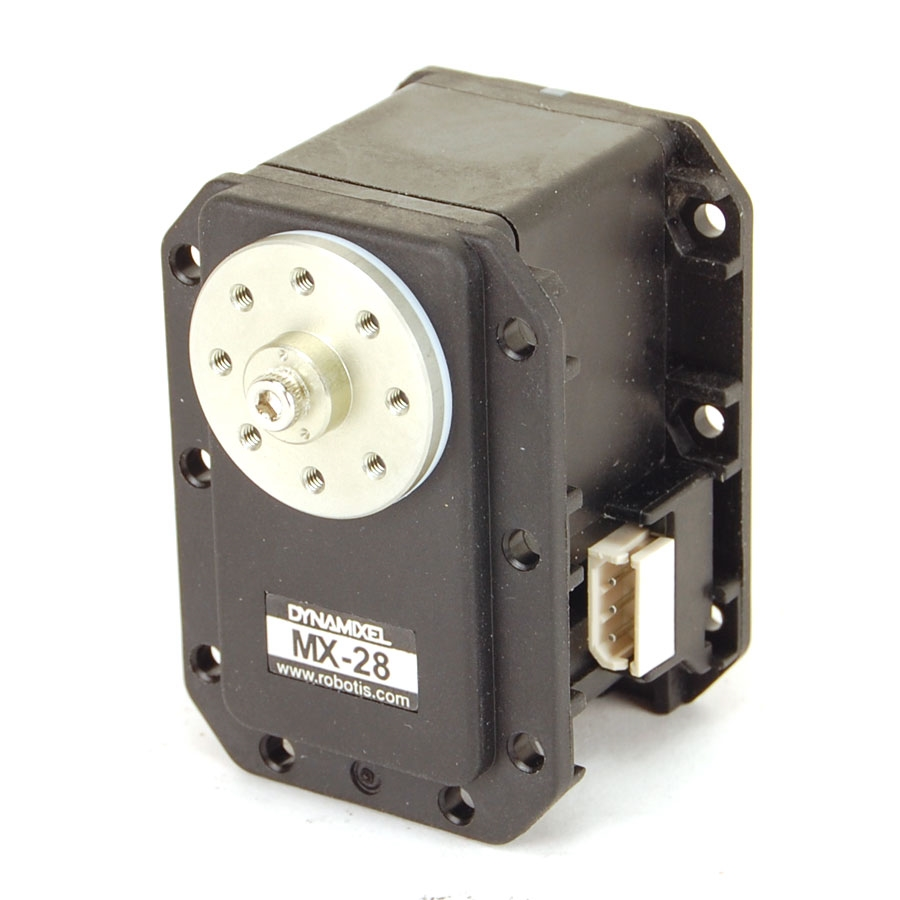
\includegraphics[width = \textwidth]{figures/mx28}
    \caption{MX-28R servo. \label{fig:mx28}}
    \end{subfigure}
    \hfill
    \begin{subfigure}[b]{0.4\textwidth}
    \center
    \includegraphics[width = \textwidth]{figures/fr07-h101}
    \caption{FR07-H101 hinge type frame. \label{fig:fr07-h101}}
    \end{subfigure}

    \begin{subfigure}[b]{0.4\textwidth}
    \center
    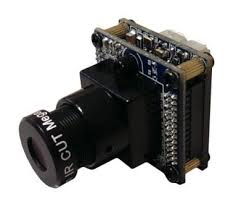
\includegraphics[width = \textwidth]{figures/li_cam}
    \caption{LI-USB30-M021C camera. \label{fig:li_cam}}
    \end{subfigure}
    \hfill
    \begin{subfigure}[b]{0.4\textwidth}
    \center
    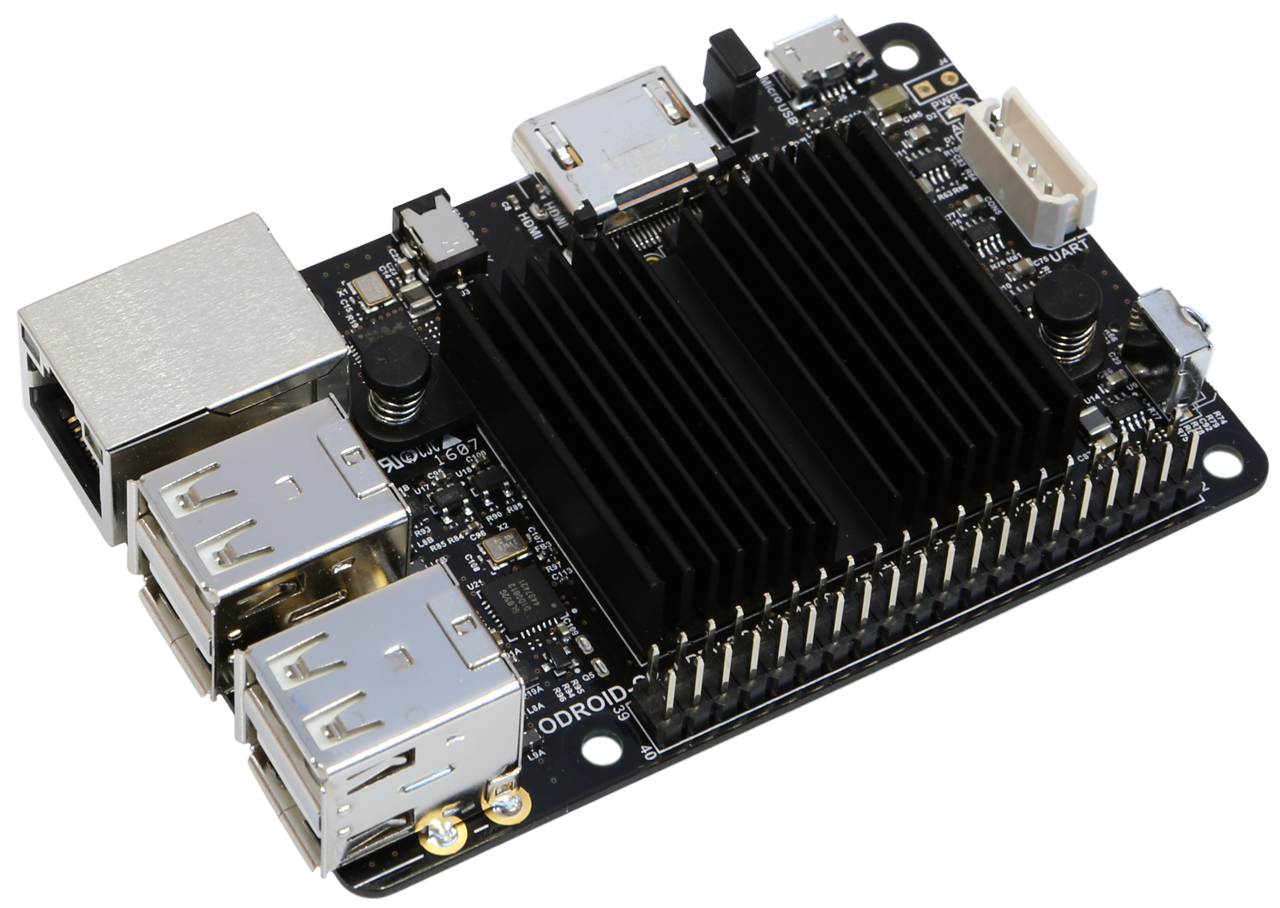
\includegraphics[width = \textwidth]{figures/odroid-c2}
    \caption{Odroid C-2 motherboard. \label{fig:odroid}}
    \end{subfigure}
    \caption[Atomic elements of our robot]{Atomic elements of our robot. The MX-28R and the camera are more complex to model as they each perform a function in the simulation. On the other hand, the frame and the motherboard are only dead weight.}
    \label{fig:modelling_problem}
\end{figure}

\section{Modelling in V-Rep \label{sec:modelling}}
The creation of a model inside V-Rep starts with the creation of a mesh\footnote{an ensemble of vertices and faces that represent an object} in a modelling tool, Blender in our case. It is preferred to have a convex mesh, i.e one that whose all interior meshes are less or equal to $180\degree$, as they are easier for the simulator to handle. When it is absolutely necessary to keep the mesh concave, a solution is to separate it into several convex meshes that will be grouped together once in V-Rep. Once saved in a file format recognized by V-Rep the mesh can be imported into the latter. 

\begin{figure}[htp]
\center
    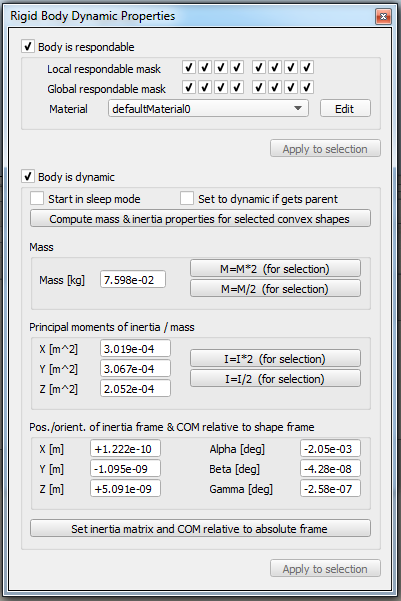
\includegraphics[width = 0.6\textwidth]{figures/v-rep_modelling}
    \caption[Rigid body dynamic properties]{Configuration window of the dynamic properties of the selected rigid body. We can make it \emph{respondable}, i.e it should collide with other objects. We can also make it \emph{dynamic} in which case it will be dynamically active in the simulation and react to forces. When dynamically active, the movement of this body will be influenced by its \emph{mass} and its \emph{inertia}. It is also possible to set what is called \emph{Material} by V-Rep.}
    \label{fig:vrep_modelling}
\end{figure}

When in V-Rep all that is left is marking the body as dynamic, respondable (if necessary) and setting the mass and the inertia. It is possible to have V-Rep compute it automatically from the geometry and the density but it can also be set manually.

\section{Modelling the miscellaneous mechanics and electronics}
The modelling of most of the mechanical elements and electronics is rather straightforward but there are some where the process is more troublesome. This is the case of the feet, frames and springs and those will be detailed hereunder after a short explanation of the modelling process of the remaining pieces.

\subsection{Modelling the electronics, batteries, hands and the central plate}
The modelling of these elements consists in following the procedure explained in \Cref{sec:modelling}. All the necessary informations are contained in \Cref{table:weights}.

\begin{table}[htp]
\center
\begin{tabularx}{\textwidth}{@{} l l X X p{4.1cm} @{}}
\toprule
\textbf{Module} & \textbf{Weight [$g$]} & \textbf{Material} &  \textbf{Density [$kg/m^3$]}& \textbf{Dimensions $x[mm] \cdot y[mm] \cdot z[mm]$}\\ 
\midrule
Odroid C-2 & 40 & [-] & 840 & $85.0 \cdot 56.0 \cdot 10.0$\\
Li-Po battery & 188 & Li-Po & 2304 & $103.0 \cdot 33.0 \cdot 24.0$\\
Hand & 30 & Aluminium & 3000 & $70.0 \cdot 31.0 \cdot 31.0$\\
Feet & 52 & Polymer & 1000 & $70.0 \cdot 125.0 \cdot 6.0$\\
Central plate & 209 & Aluminium & 4000 & $140.0 \cdot 30.0 \cdot 124.5$\\
\bottomrule
\end{tabularx}
\caption[Weights and dimensions of the pieces of the robot]{Weights and dimensions of the pieces of the robot. The density is useful for the automatic computation of the weight and inertia of the pieces in V-REP. The differences in density between different pieces made of the same material represent the differences in geometry, i.e pieces with holes in them that are not modelled but taken into account by making the piece lighter.}
\label{table:weights}
\end{table}

\subsection{Modelling the feet}
In essence, the feet of our robot will be plates that will be fixed to the last servos of the legs. Contrary to other elements, feet \emph{must} be respondable as they come into contact with the floor. It follows that the friction parameter will be important too and it will have to be chosen in accordance to the friction parameter of the material they will be made of.

It should be noted that for the needs of the simulation, their z dimension has been exaggerated up to $6mm$ because of collision problems (sometimes, the contact point was on the upper side of the feet while it should have been on the down side) that disturbed the course of the simulation. Therefore, the z dimension reported in \Cref{table:weights} is the double of the actual one and the density has been halved to keep the same mass.

\subsection{Frames}
Frames are a special case: in the actual robot they are essential in connecting the servos together but they are not necessary in the simulation. Indeed the link between servos can be made directly through the joints without the intermediary of a frame. 

This reduces the accuracy of the model but not by much and we gain in speed and stability by reducing the number of constraints and not having to integrate a convex shape into the model.

\subsection{Springs}
By itself a spring can be modelled by a prismatic joint linking two dynamic objects together. The prismatic joint is then set to \emph{spring-damper} mode and the stiffness and damping can be specified.

However, if we want to add it to a leg we have to somehow create a loop in a top down hierarchy. Moreover, we need to take into account displacements of the anchors. 
\begin{figure}[htp]
\center
    \begin{subfigure}[b]{0.45\textwidth}
    \center
    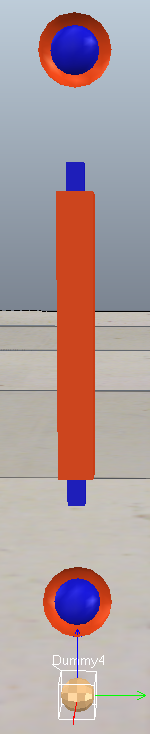
\includegraphics[height = 0.5\textwidth]{figures/springs}
    \end{subfigure}
    \hfill
    \begin{subfigure}[b]{0.45\textwidth}
    \center
    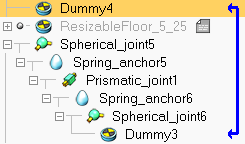
\includegraphics[height = 0.5\textwidth]{figures/springs_hierarchy}
    \end{subfigure}
\caption[Model of a spring inside V-Rep]{How to model a spring inside V-Rep. }
\label{fig:springs}
\end{figure}

\section{Modelling the cameras}
The robot will be equipped with two small cameras, of the type illustrated in \cref{fig:camera}, used to locate the robot on the field\footnote{This is the subject of another master's thesis this year.}. 

We model the hull of the camera as cube. The dimensions and weight are in \cref{table:weights}. We model the active part of the camera as a \emph{vision sensor}, a V-Rep object that simulates cameras. It can be customized to have the desired resolution, field-of-view, ...

That image sensor can be reached through the remote API of V-Rep in a number of ways : \begin{itemize}
\item Streaming : the data from the vision sensor can be sent continuously to the control code but this slows down the simulation significantly. V-Rep supports streaming, reducing the communication overhead.
\item Oneshot : we can request one image from the simulator. This is less expensive and will probably be preferred.
\end{itemize} 

All the characteristics of the model of a camera are compiled in \cref{table:cam_specs}.

\begin{table}[htp]
\center
\begin{tabularx}{\textwidth}{@{}X X X @{}}
\toprule
 & \textbf{Data} & \textbf{Unit}\\ 
\midrule
Weight & 22 & $g$\\
Dimensions & 26.0 x 26.0 x 14.7 & $mm^3$\\
Density & 2213 & $kg/m^3$\\
Inertia & & $gmm^3$\\
Resolution &  & $px^2$\\
Field of view & & $\degree$\\
\bottomrule
\end{tabularx}
\caption[Characteristics of the LI-USB30-M021C camera]{Characteristics of the model of the LI-USB30-M021C camera}
\label{table:cam_specs}
\end{table}

\section{Modelling the MX-28R}
This section explains how the MX-28R is characterized and modelled.

\subsection{Determining the continuous torque}
The primary parameter we must know the value of to properly model the MX-28R is the torque it generates. The manual (\cite{mx_28_manual}) provides the value of the stall torque ($2.5Nm$ @$12V$) and a graph showing the efficiency of the servo at different torques and speeds but it does not provide a value of the actual continuous torque. We thus compute it from the maximal torque of the DC motor (référence à mettre !) and the reduction ratio of the gears. 
\begin{align*}
ContinuousTorque &= TorqueMotor \times ReductionRatio\\
&= 3.67e^{-3} \times 193\\
&= 0.7083Nm
\end{align*}
The continuous torque is thus equal to $0.7Nm$.

\subsection{Determining the stall torque}
The stall torque is determined through a small experiment with a real MX-28R. The experimental setup is explained in \Cref{fig:exp_setup} and \Cref{fig:usb2dyn}. The experiment itself is presented in \Cref{fig:exp1}.

\begin{figure}[htp]
\center
    \begin{subfigure}[b]{0.45\textwidth}
    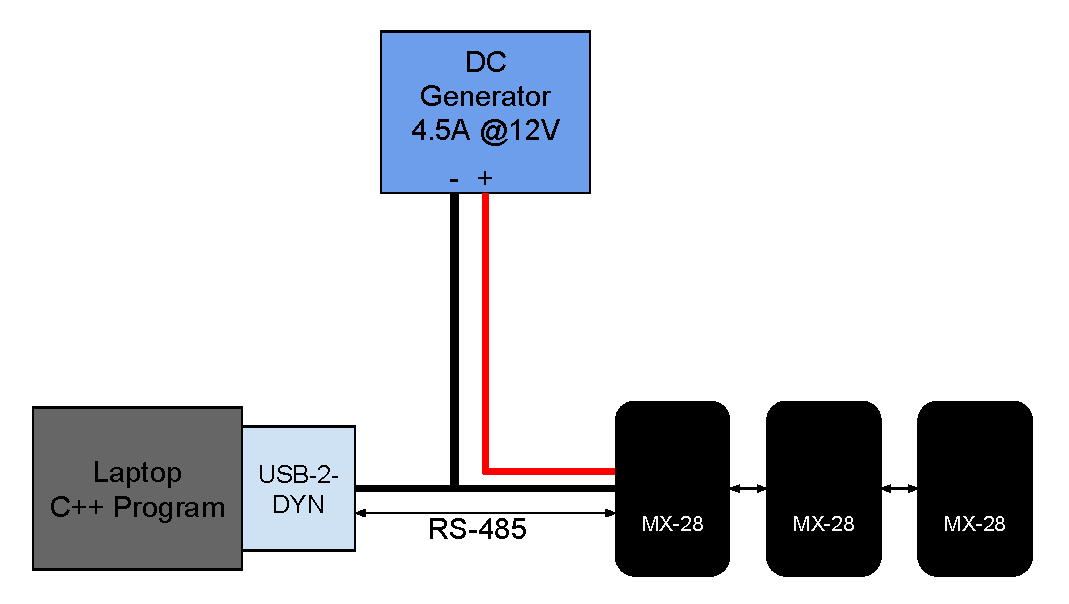
\includegraphics[width=\textwidth]{figures/exp_setup}
    \caption[Experimental setup]{The MX-28 servos are powered by a DC generator and controlled by a laptop equipped with a USB2DYNAMIXEL(USB-2-DYN) device.}
    \label{fig:dc_chain}
    \end{subfigure}
    \hfill
    \begin{subfigure}[b]{0.45\textwidth}
    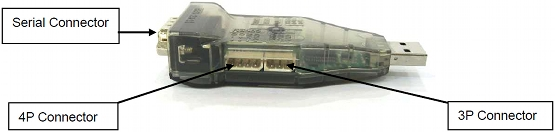
\includegraphics[width = \textwidth]{figures/u2d}
    \caption[USB2DYNAMIXEL]{A USB2DYNAMIXEL. It turns an USB port into a serial port (RS485, TTL or classic serial connector) that can be used to control Dynamixel manufactured servos. [Photo from \cite{usb2dyn_manual}]}
    \label{fig:usb2dyn}
    \end{subfigure}
    \caption{Experimental setup \label{fig:exp_setup}}
\end{figure}

\begin{figure}[htp]
\center
    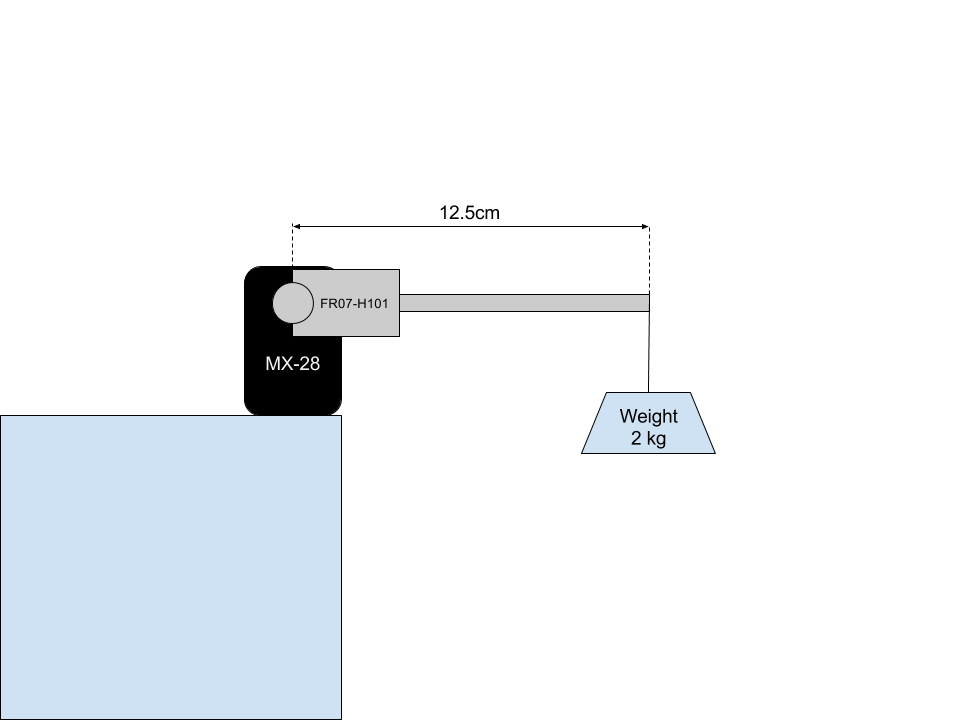
\includegraphics[width = 0.5\textwidth]{figures/exp1}
    \caption[Experimental setup for torque testing]{Experimental setup for torque testing. A weight $w$ of is suspended at a distance $d$ from the servo, resulting in a applied torque of $w \times g \times d$. The goal is to find the weight $w$ for which the servo is unable to lift the arm.}
    \label{fig:exp1}
\end{figure}

\begin{figure}[htp]
\center
    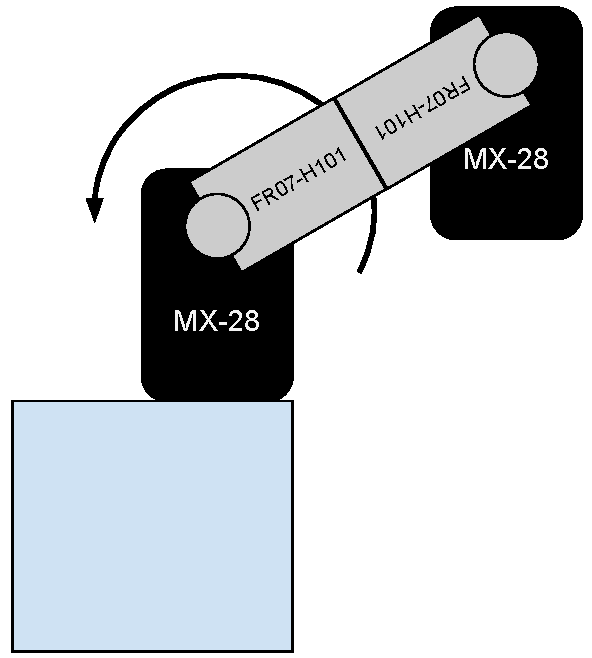
\includegraphics[width = 0.3\textwidth]{figures/exp2}
    \caption[Experimental setup dynamics testing]{Experimental setup for dynamics testing. One servo lifts the other. The goal is the measure the time it takes to swing the arm from $0\degree$ to $180\degree$.}
    \label{fig:exp2}
\end{figure}

In our case, $d$ was equal to $22.5cm$ and we could reach a weight $w$ of $740g$ at $14.8V$. This equals to a torque of $1.64Nm$. The complete results are listed in \Cref{table:mx28-specs}.

\subsection{Determining the rotation speed}
In this experiment we will test some simple dynamics. The setup is shown in \cref{fig:exp2}. The goal is to tune the P parameter of the PID controller inside V-Rep. In order to achieve this, we film the real servo going from $0\degree$ to $180\degree$ and measure the time it takes. 

Executing this manoeuvre at $12V$ with no speed limit imposed takes $620msec$.

We then reproduce the same manoeuvre inside V-Rep, measuring the time through code. We modify the proportional gain of the PID controller until we get the same time.



\subsection{Results}
\begin{table}[htp]
\begin{tabularx}{\textwidth}{@{} l X X @{}}
\toprule
& \textbf{Data} & \textbf{Unit}\\ 
\midrule
Weight & $77$ & $g$\\
Dimensions & $35.6 \times 50.6 \times 35.5$ & $mm^3$\\
Ixx & $22,649$ & $g \cdot mm^4$\\
Iyy & $12,868$ & $g \cdot mm^4$\\
Izz & $17,733$ & $g \cdot mm^4$ \\
Announced stall torque @11.1V & $2.1$ & $Nm$\\
Experimental stall torque @11.1V & $1$ & $Nm$\\
Announced stall torque @12V & $2.5$ & $Nm$\\
Experimental stall torque @14.8V & $1.2$ & $Nm$\\
Announced stall torque @14.8V & $3.1$ & $Nm$\\
Experimental stall torque @12V & $1.6$ & $Nm$\\
Nominal continuous torque @12V & $0.7$ & $Nm$\\
Announced unloaded rotation speed @12V & $55.00$ & $Rpm$\\
Experimental unloaded rotation speed @12V & $48.33$ & $Rpm$\\
\bottomrule
\end{tabularx}
\caption[]{Characteristics of a MX-28R type servo. Data taken from \cite{mx_28_manual} and from \url{http://www.robotis.com/view/DXL-INERTIA/RX-28_INERTIA.pdf}[Accessed 4/6/2016].}
\label{table:mx28-specs}
\end{table} 

\subsection{Modelling the MX-28R}
\begin{figure}[htp]
\center
\begin{subfigure}[b]{0.3\textwidth}
    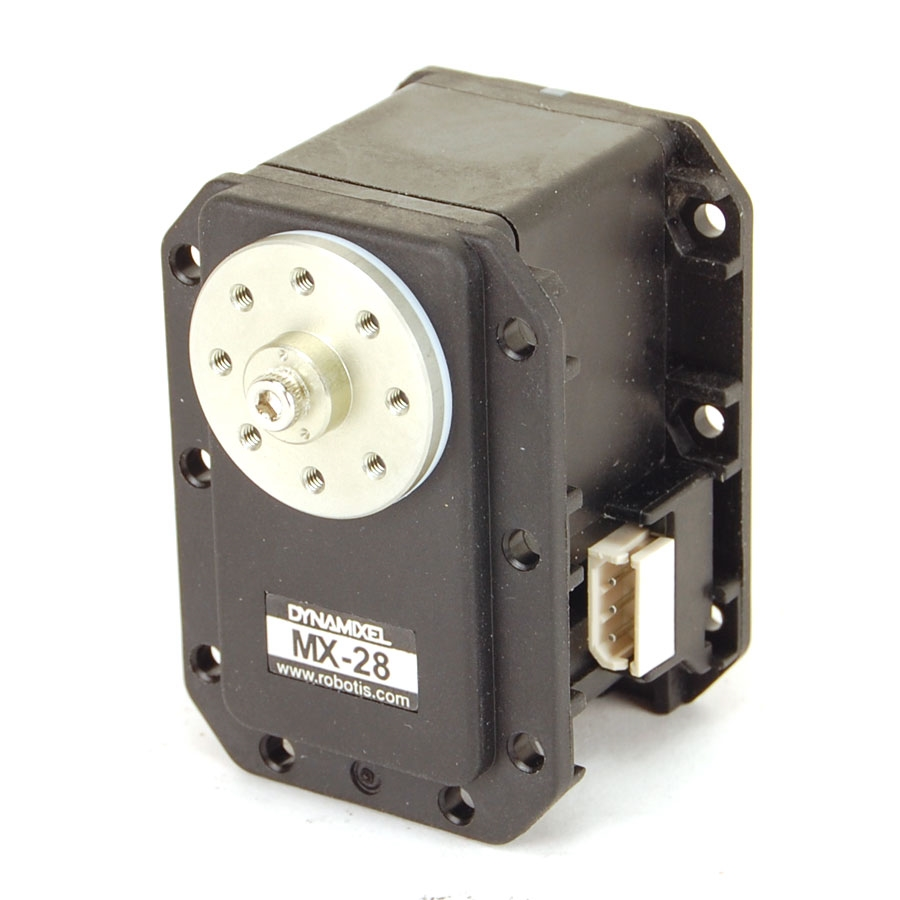
\includegraphics[width = \textwidth]{figures/mx28}
    \caption{MX-28R servo.}
    \label{fig:mx28_real}
\end{subfigure}
\hfill
\begin{subfigure}[b]{0.3\textwidth}
    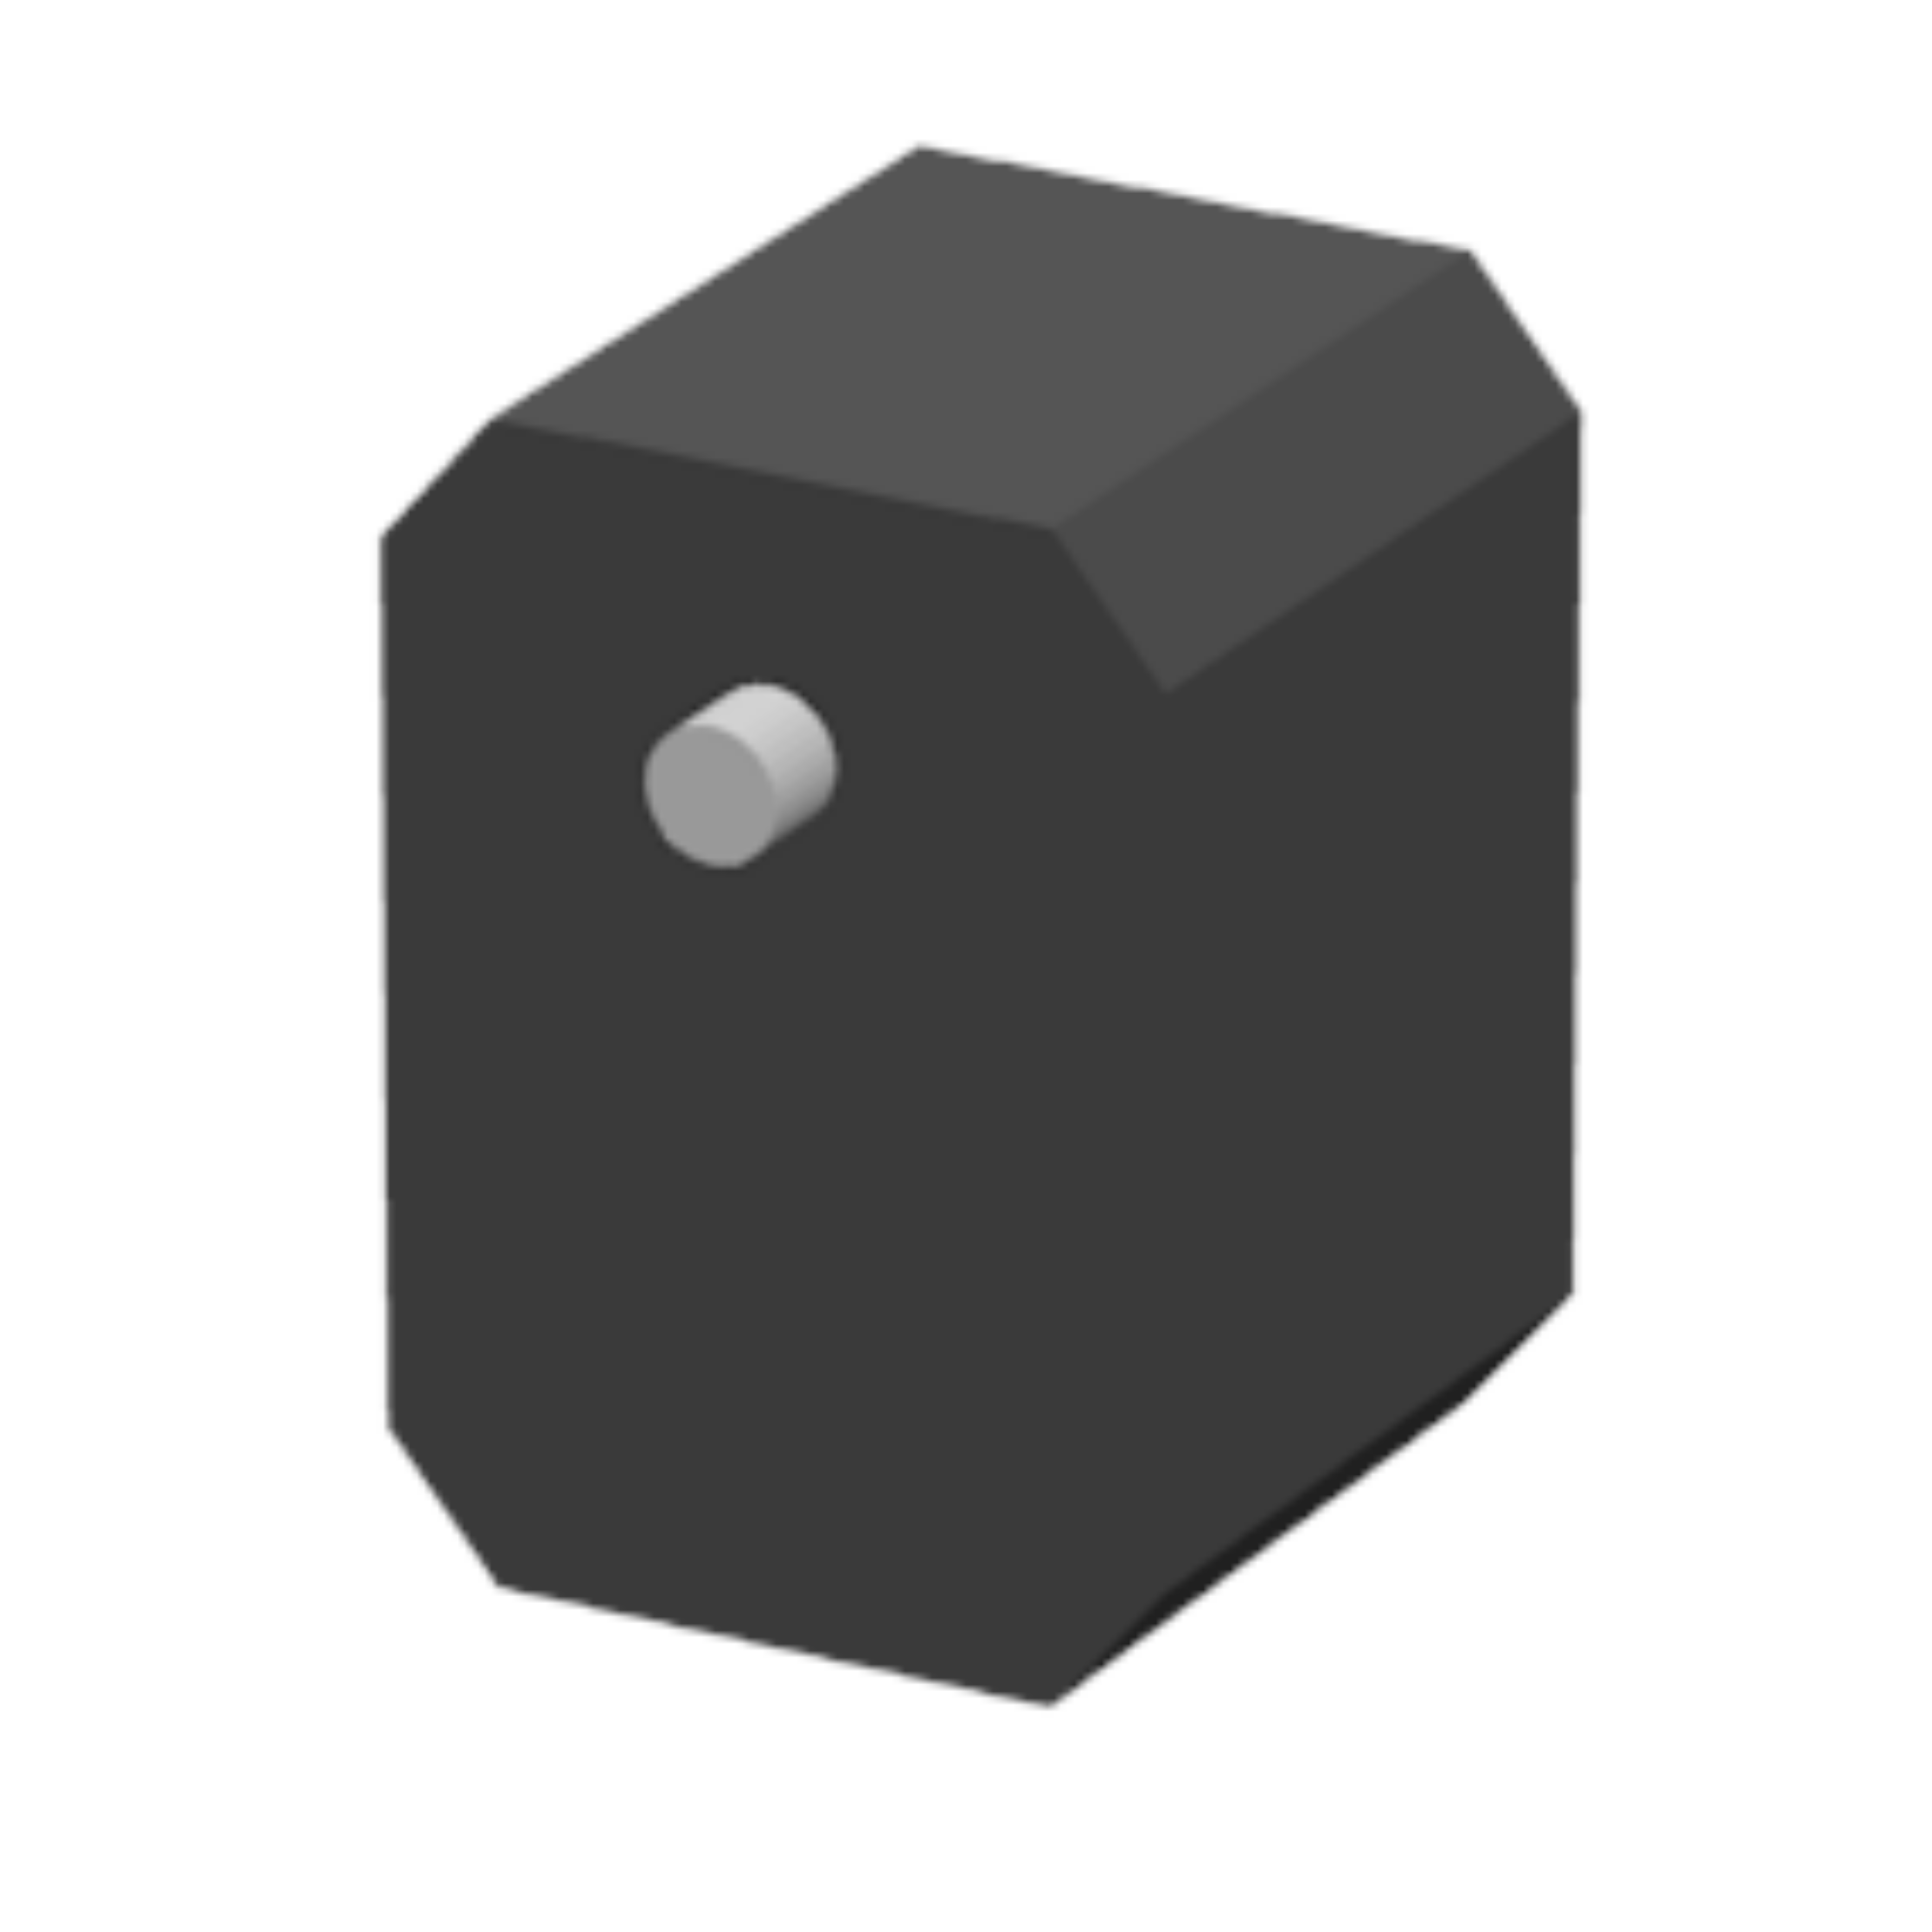
\includegraphics[width = \textwidth]{figures/mx28_model}
    \caption{Model of the MX-28R.}
    \label{fig:mx28_model}
\end{subfigure}
\caption[Side by side of a MX-28R servo and its 3D model]{Side by side of a MX-28R servo and its 3D model. The shape has been simplified but retains outer appearance of the servo. The axis is used as a position marker and will be removed once the joints are in place.}
\label{fig:servo}
\end{figure}

In V-Rep the different elements of the robot are dynamically enabled and given mass, accordingly to the values listed in \cref{table:weights}. Then, joints (motor controlled with control loop activated) are added to simulate the behaviour of the servos. Their maximal torque is set to $1.2$, the maximum torque developed my Mx-28 servos as shown by our earlier experiments (\cref{table:exp1_results}). 

The original MX-28R servo does not have any accelerometer, but a master's thesis in progress is going to change that. We can emulate it in the simulator by differentiating the position, obtained through \emph{simxGetObjectPosition}. 

\begin{figure}[htp]
\center
    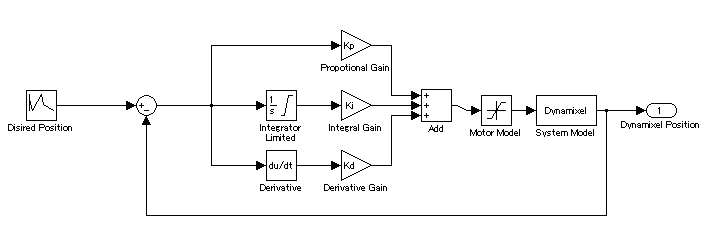
\includegraphics[width = \textwidth]{figures/pidcontrol}
    \caption[MX-28 PID controller]{MX-28 PID controller, as represented in \cite{mx_28_manual}. It is a standard PID controller although by default only the P parameter is non-zero. The function of the \textit{motor model} block is to clamp the computed correction torque in the allowed interval whereas the \emph{system model} block is a simulink representation of the MX-28R and does not exist in the actual implementation inside the latter.}
    \label{fig:mx28_pid}
\end{figure}